\section{One-dimensional Advection-Diffusion Equation}
\label{sec: exp-1d}

The preceding rotating-hill example established the behaviour of the complete adaptive workflow for a manufactured space--time tracking functional. We now turn to a one-dimensional advection--diffusion problem that provides a more controlled setting for examining the role of the quantity of interest. In this test, the primal problem and localisation procedure are kept fixed while the location of an observation sensor is varied. Any resulting change in the refinement pattern can therefore be attributed to the goal functional, through its associated dual weight. Moreover, since the problem is spatially one-dimensiona, its space--time mesh can be displayed directly in the \((x,t)\) plane, allowing spatial and temporal refinement to be viewed simultaneously.


\subsection{Primal Problem}

We consider the advection--diffusion equation
\begin{equation}
  \partial_t u
  - \varepsilon\,\partial_{xx}u
  + b\,\partial_xu
  = f
  \qquad
  \text{in }(0,1)\times(0,T),
  \label{eq:advection-diffusion-1d}
\end{equation}
subject to homogeneous Dirichlet boundary conditions
\begin{equation}
  u(0,t)=u(1,t)=0,
  \qquad t\in(0,T],
\end{equation}
and the initial condition
\begin{equation}
  u(x,0)
  =
  x(1-x)
  \exp\!\left[-\beta(x-x_0)^2\right].
\end{equation}
The forcing term $f$ is manufactured so that the exact solution is
\begin{equation}
  u_{\rm{ex}}(x,t)
  =
  x(1-x)
  \exp\!\left[
    -\beta\bigl(x-x_0-bt\bigr)^2
  \right].
  \label{eq:moving-pulse}
\end{equation}
The parameters used throughout the experiments are
\begin{equation*}
  \varepsilon=0.02,
  \qquad
  b=0.6,
  \qquad
  \beta=100,
  \qquad
  x_0=0.2,
  \qquad
  T=1.
  % \label{eq:advection-diffusion-parameters}
\end{equation*}

The solution represents a narrow concentration pulse transported from left to right while undergoing diffusion. Its nominal centre follows the trajectory
\begin{equation*}
  x_c(t)=x_0+bt=0.2+0.6t
\end{equation*}
and therefore reaches $x_c(T)=0.8$ at the final time. 
% The factor $x(1-x)$ ensures compatibility with the homogeneous boundary conditions and causes the amplitude of the pulse to vary as it moves through the domain. 
Figure~\ref{fig:advection-diffusion-exact} shows the resulting space--time solution.

\begin{figure}[h]
  \centering
  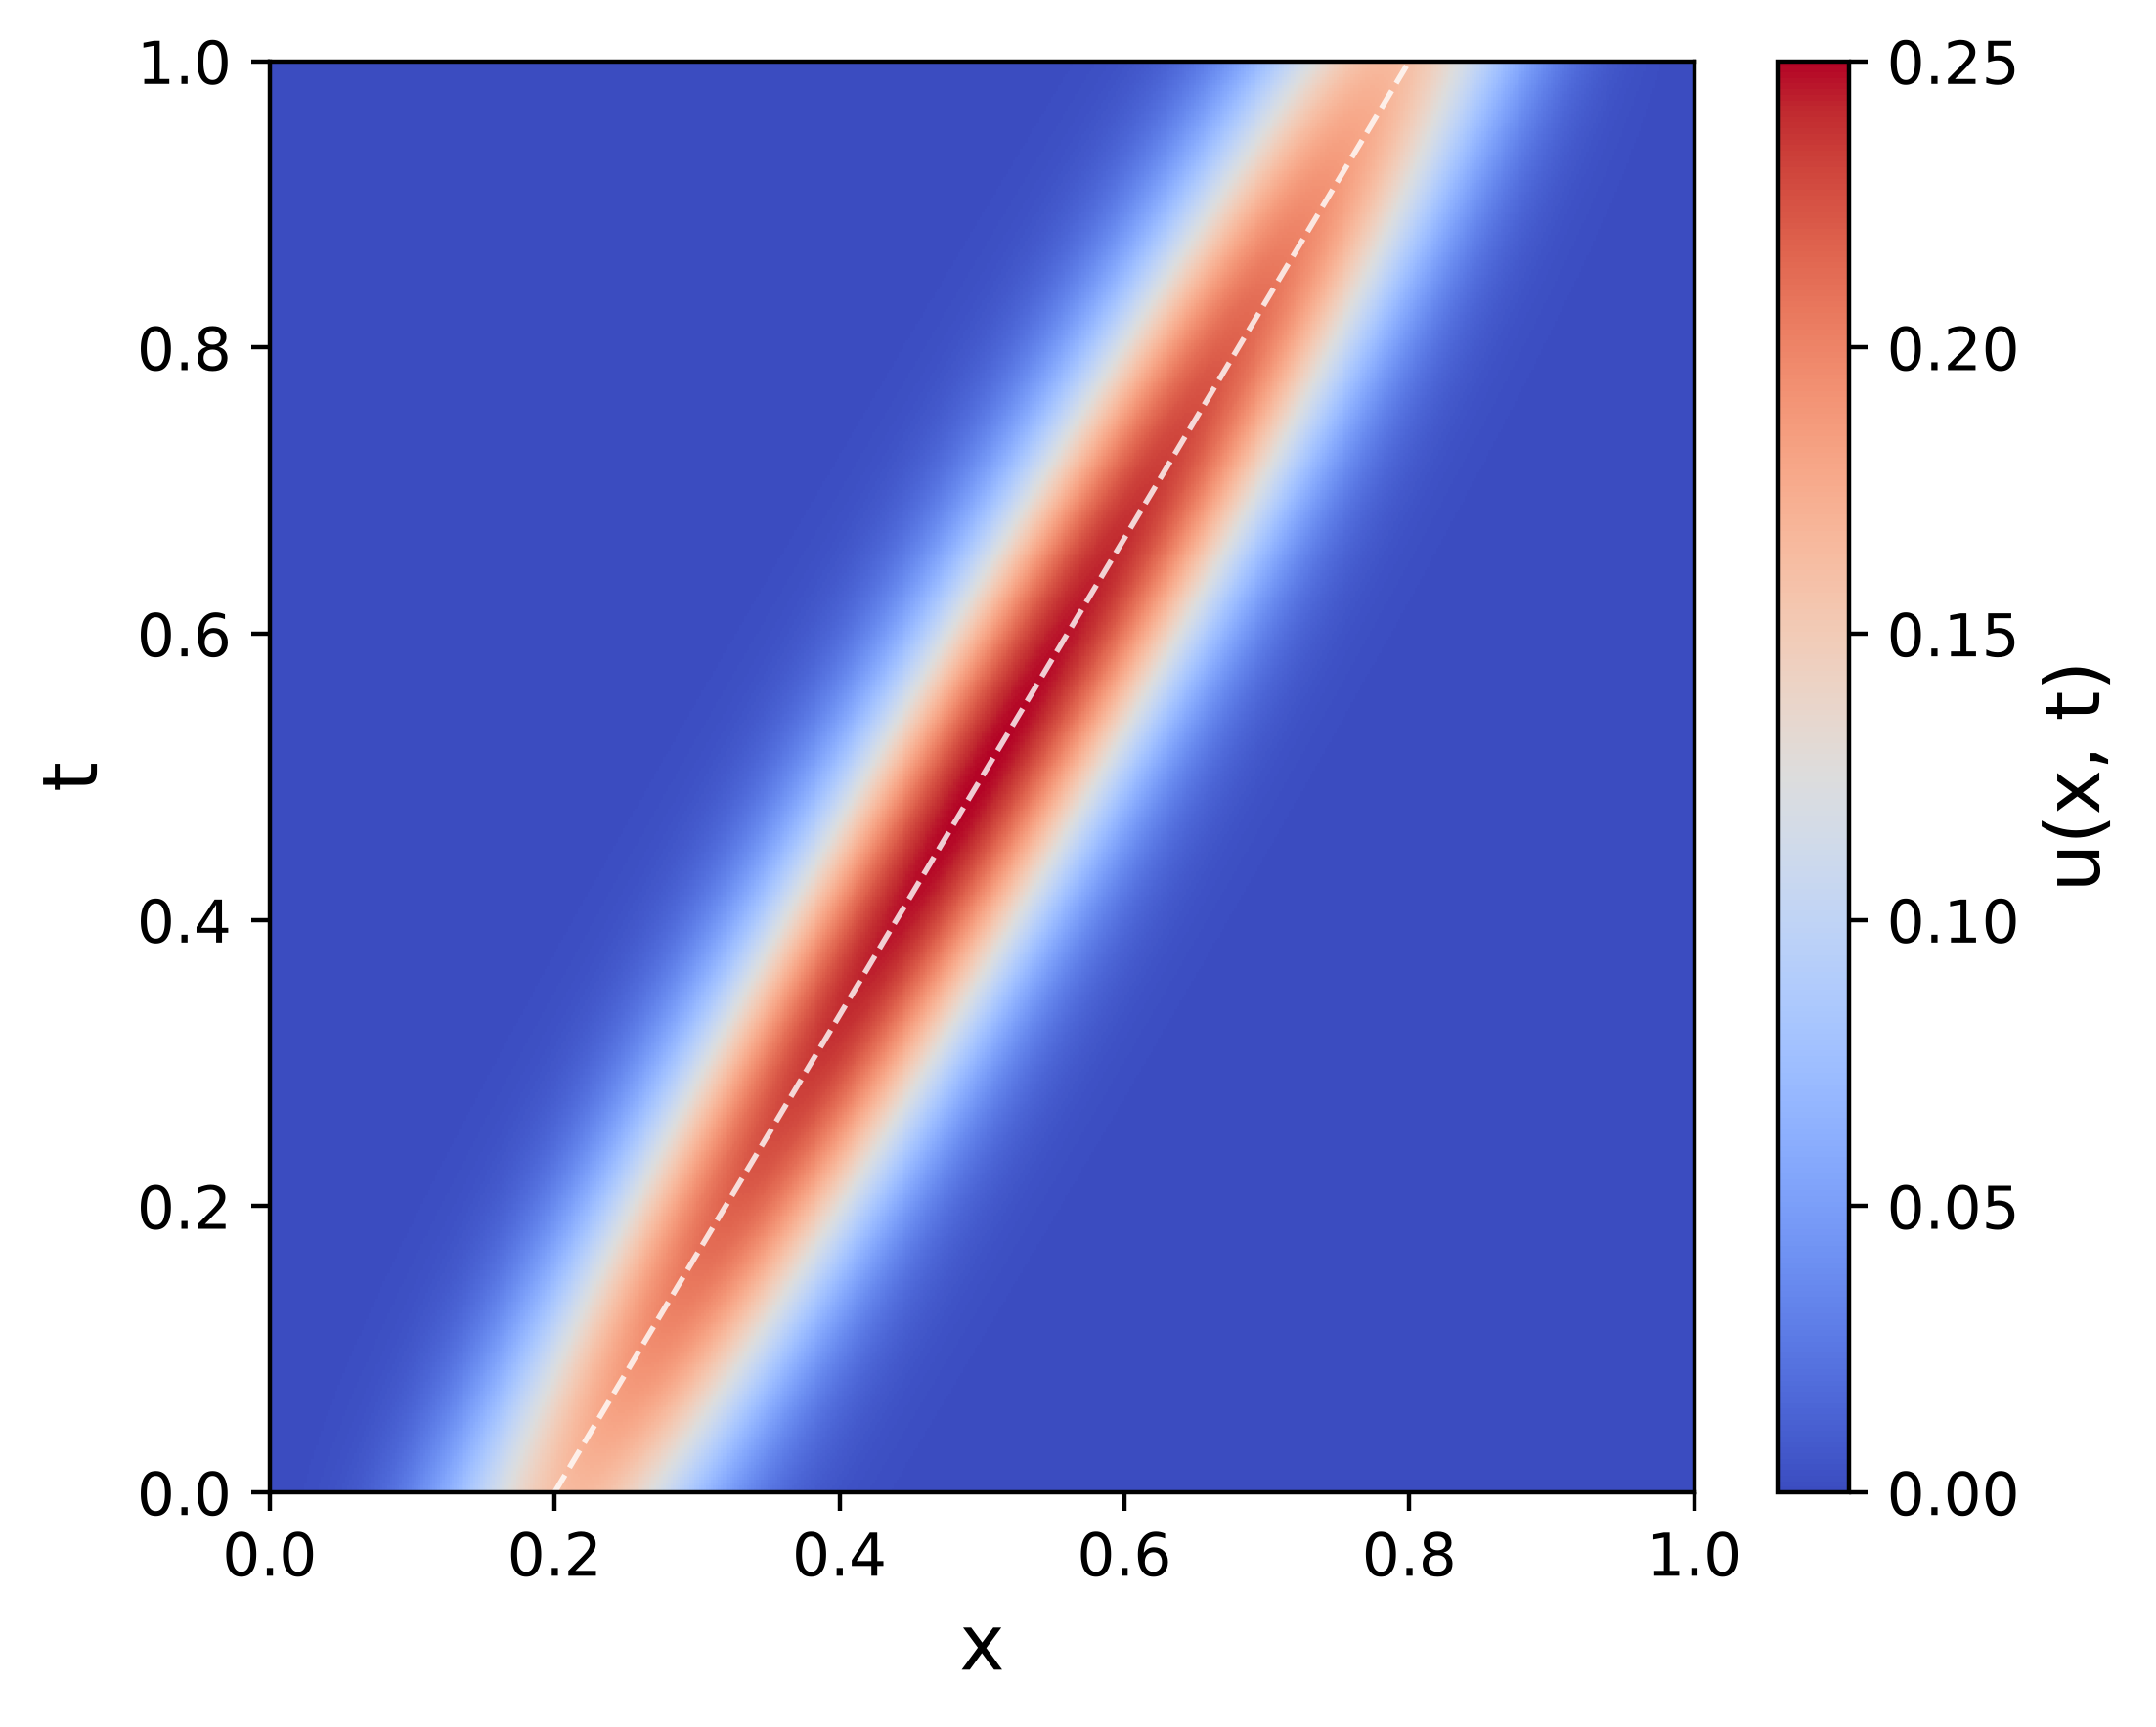
\includegraphics[
    width=0.45\textwidth
  ]{figures/advection_diffusion_1d/advection_diffusion_exact_solution.png}
  \caption{Exact solution of the 1D advection--diffusion problem. The dashed line indicates the nominal pulse trajectory.}
  \label{fig:advection-diffusion-exact}
\end{figure}


\subsection{Quantity of Interest and Adjoint Sensitivity}

To study the influence of the goal functional, we introduce a family of finite-width terminal detectors,
\begin{equation}
  J_{x_d}(u)
  =
  \int_0^1
  \psi_{x_d}(x)\,u(x,T)\,\mathrm{d}x,
  \qquad
  \psi_{x_d}(x)
  =
  \exp\!\left[
    -\left(\frac{x-x_d}{r_d}\right)^2
  \right],
  \label{eq:qoi-gaussian-family}
\end{equation}
where
\begin{equation}
  r_d=0.05,
  \qquad
  x_d\in\{0.7,0.8,0.9\}.
  \label{eq:sensor-locations}
\end{equation}
The goal functional can be interpreted as the response of a sensor whose sensitivity is maximal at $x_d$ and decreases smoothly away from its centre. The adjoint \(z\) associated with \(J_{x_d}\) satisfies
\begin{equation}
-\partial_t z
-\varepsilon\partial_{xx}z
-b\partial_xz
=0
\qquad
\text{in }(0,1)\times(0,T),
\label{eq:advection-diffusion-adjoint}
\end{equation}
with homogeneous boundary conditions and terminal datum
\begin{equation}
z(x,T)=\psi_{x_d}(x).
\label{eq:advection-diffusion-adjoint-terminal}
\end{equation}
Thus, the detector location determines where the adjoint sensitivity is concentrated at the final time. The behaviour of this sensitivity is most easily understood in reversed time \(\tau=T-t\), for which the adjoint equation becomes
\begin{equation}
\partial_\tau z
-\varepsilon\partial_{xx}z
-b\partial_xz
=0,
\qquad
z(x,0)=\psi_{x_d}(x).
\label{eq:advection-diffusion-adjoint-reversed-time}
\end{equation}
Hence, as the adjoint is propagated backwards in physical time, its terminal Gaussian is transported to the left and broadened by diffusion. Away from the boundaries, its centre approximately follows
\begin{equation}
x_z(t)\approx x_d-b(T-t).
\label{eq:advection-diffusion-adjoint-centre}
\end{equation}

The three detector locations therefore generate three parallel, spatially shifted sensitivity trajectories in the \((x,t)\) plane. Since the primal problem is identical in all three runs, differences in the adapted meshes can be attributed to these shifted dual weights. The resulting refinement is expected to reflect the interaction between the forward pulse-error trajectory and the detector-dependent adjoint-sensitivity band.


\subsection{One-dimensional Residual Localisation}
\label{sec:one-dimensional-localisation}

The residual localisation requires a minor modification in one spatial dimension. In higher dimensions, the localised residual generally contains cell-interior contributions and contributions supported on spatial facets. In one dimension, however, the facets of an interval are its two endpoints. The facet contribution therefore is represented by point evaluations at the left and right endpoints rather than by integration over edges or faces of positive dimension.

On each space--time cell
\(
  K\times I_n,
  \,\,
  I_n=(t_{n-1},t_n],
\)
the local indicator is decomposed as
\begin{equation}
  \eta_{K,n}
  =
  \eta_{K,n}^{\mathrm{vol}}
  +
  \eta_{K,n}^{\mathrm{end}}
  +
  \eta_{K,n}^{\mathrm{time}},
  \label{eq:1d-local-indicator-decomposition}
\end{equation}
where $\eta_{K,n}^{\mathrm{vol}}$ is the cell-interior contribution, $\eta_{K,n}^{\mathrm{end}}$ contains the spatial endpoint contributions, and $\eta_{K,n}^{\mathrm{time}}$ represents the residual at the left temporal interface of the slab.


\subsection{Results and Interpretation}

In this numerical test, the initial discretisation contains $12$ spatial cells and $8$ time slabs. The primal solution and numerical dual use cG1 in space and dG0 in time. The enriched dual uses the corresponding higher-order space--time approximation. A marking parameter \(\theta=0.6\) is used and a time slab is bisected when the fraction of its marked spatial cells is at least \(15\%\).

First of all, \cref{fig:advection-diffusion-evolution} shows the evolution of the space--time mesh for the central sensor at $x_d=0.8$. Refinement is concentrated around the transported pulse and occurs in both the spatial and temporal directions.
\begin{figure}[h]
  \centering
  % space--time axis
  \begin{subfigure}[h]{0.05\textwidth}
    \centering
    \begin{tikzpicture}[>=latex, line width=0.6pt, scale=0.8]
      \draw[->] (0,0) -- (0,0.6) node[above=1pt] {$t$};
      \draw[->] (0,0) -- (0.6,0) node[below=1pt] {$x$};
    \end{tikzpicture}
    \vspace{-2em}
    \captionsetup{labelformat=empty}
    \caption{}
  \end{subfigure}
  \hfill
  \begin{subfigure}[h]{0.30\textwidth}
    \centering
    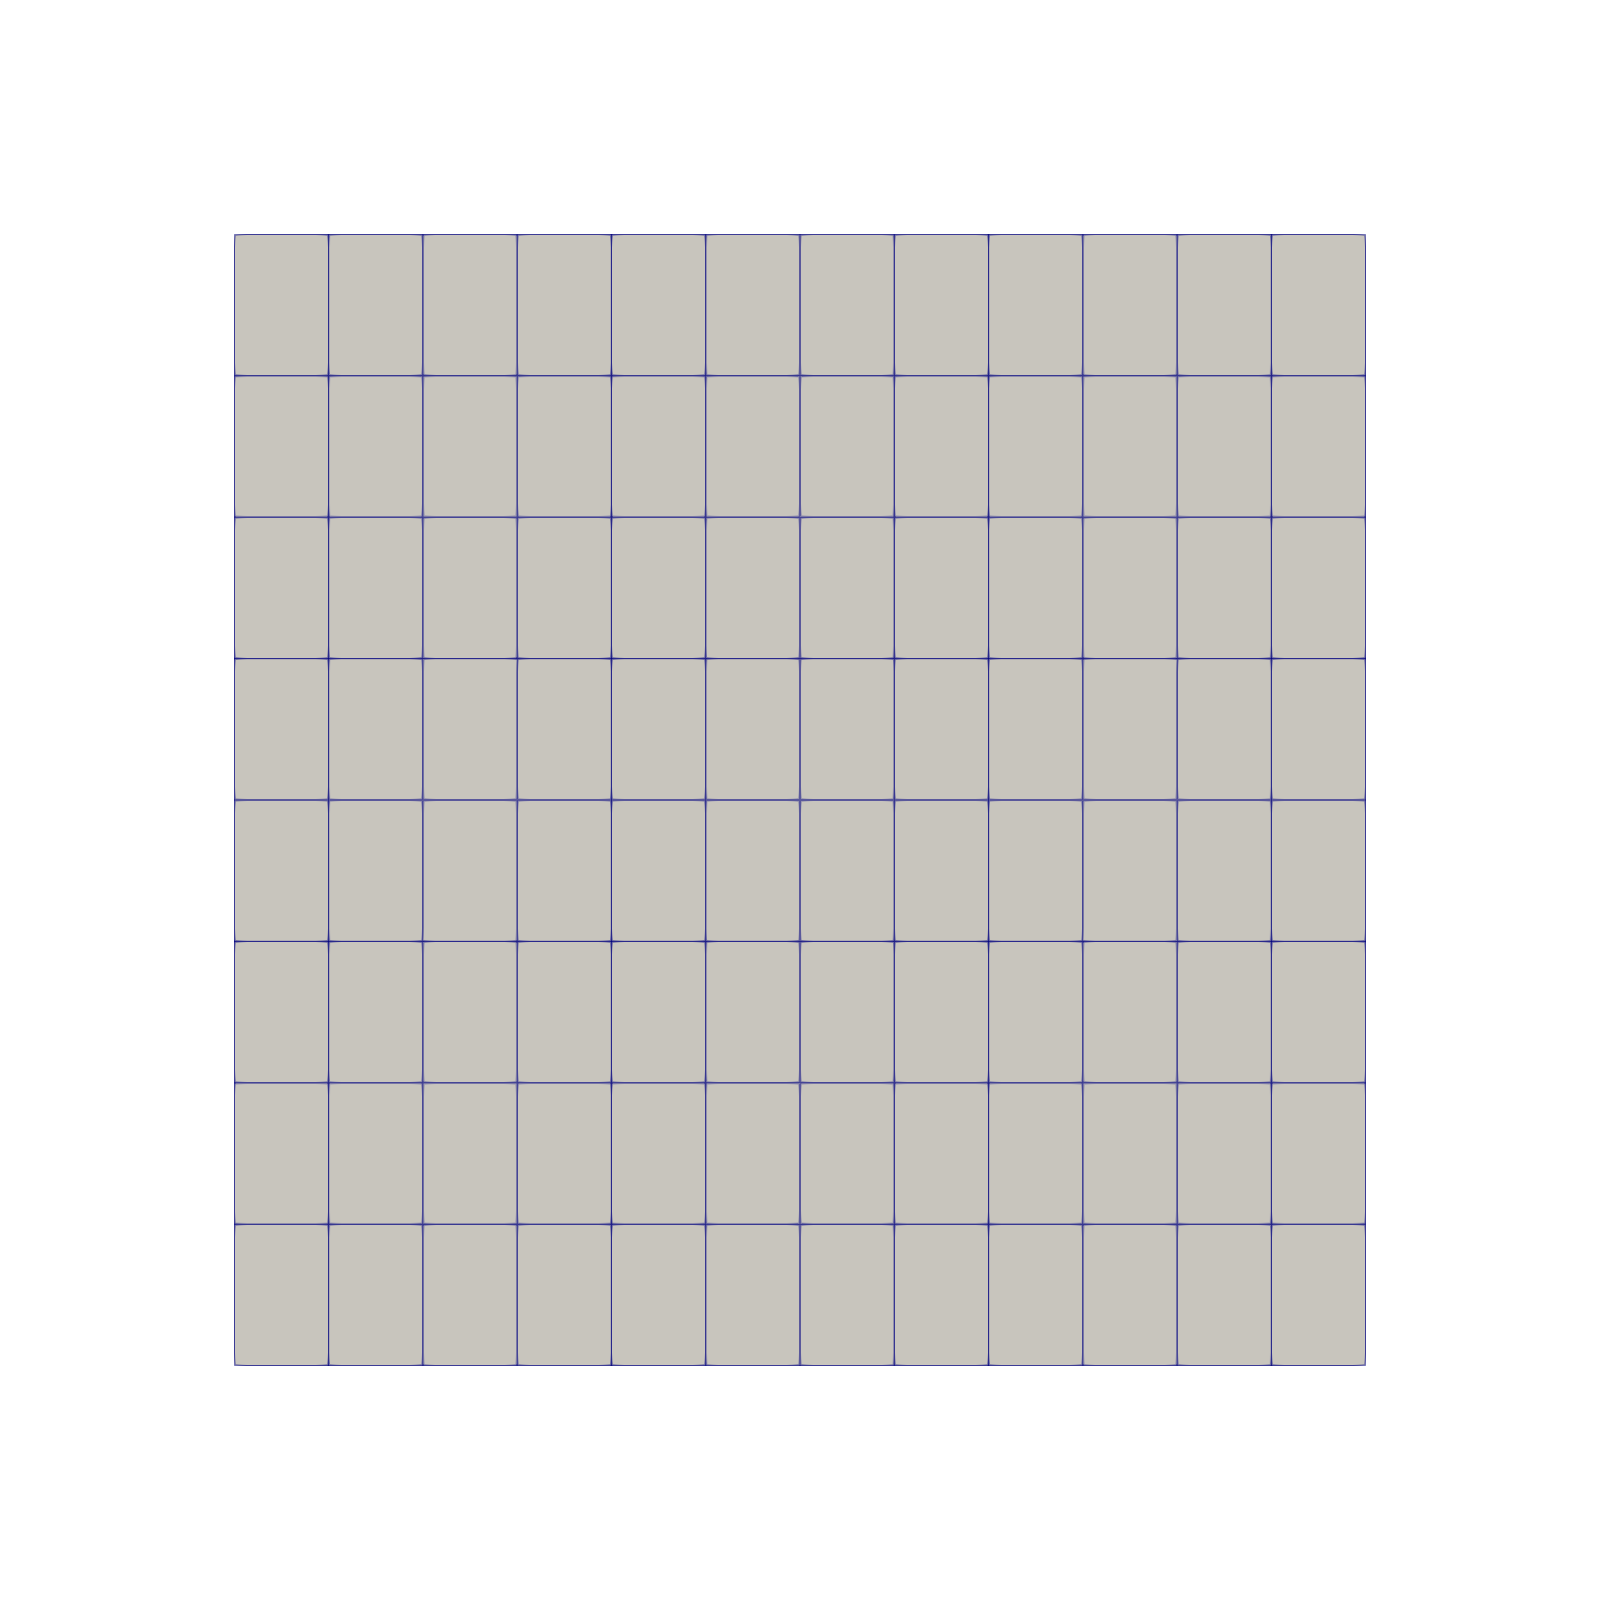
\includegraphics[
      width=\linewidth
    ]{figures/advection_diffusion_1d/mesh_x080_iter.0000.png}
    \caption{Iteration 0.}
  \end{subfigure}
  \hfill
  \begin{subfigure}[h]{0.30\textwidth}
    \centering
    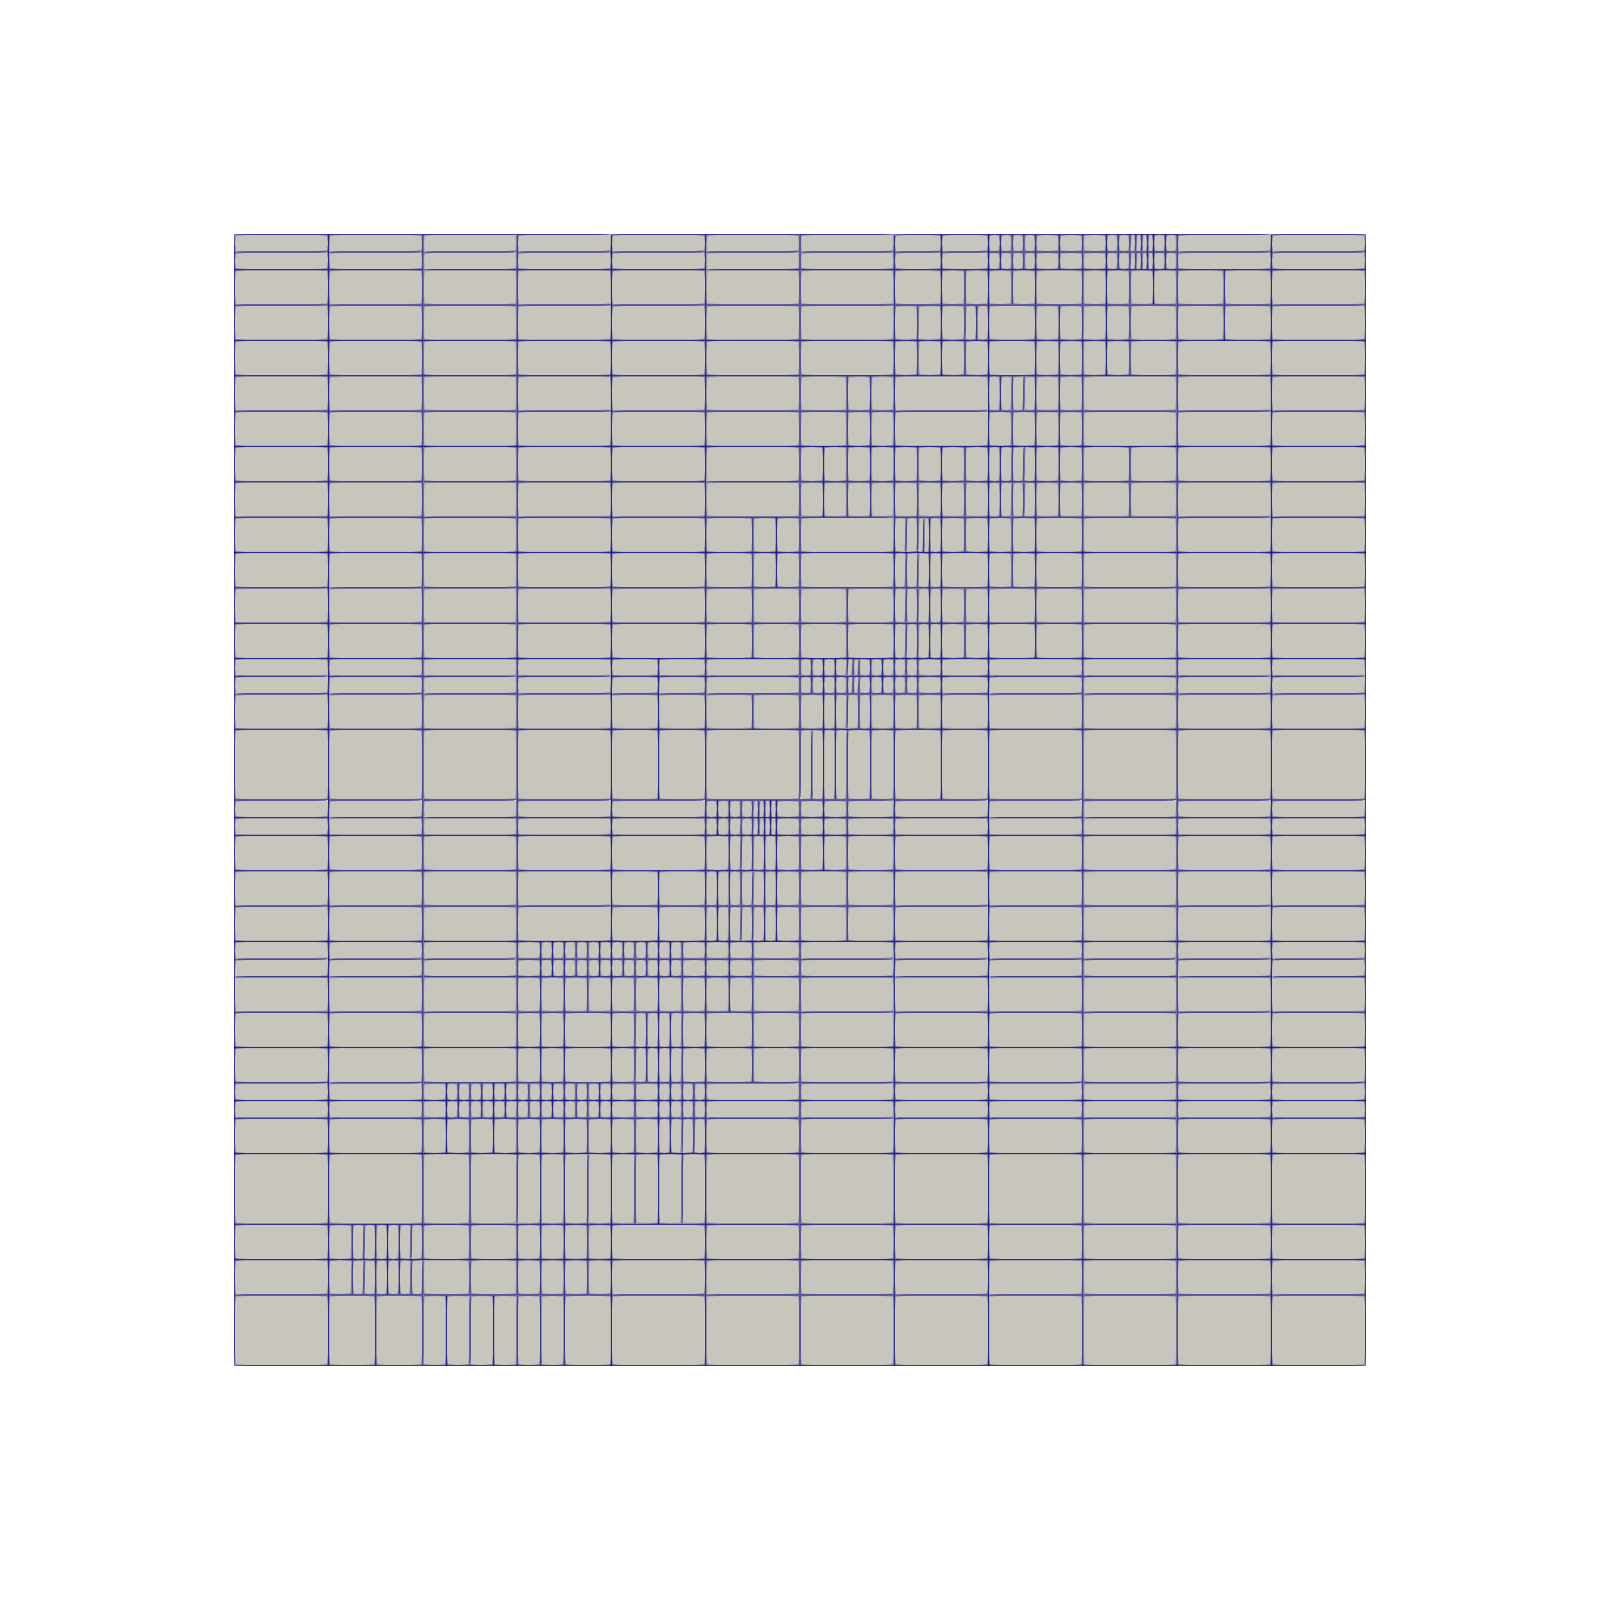
\includegraphics[
      width=\linewidth
    ]{figures/advection_diffusion_1d/mesh_x080_iter.0004.png}
    \caption{Iteration 4.}
  \end{subfigure}
  \hfill
  \begin{subfigure}[h]{0.30\textwidth}
    \centering
    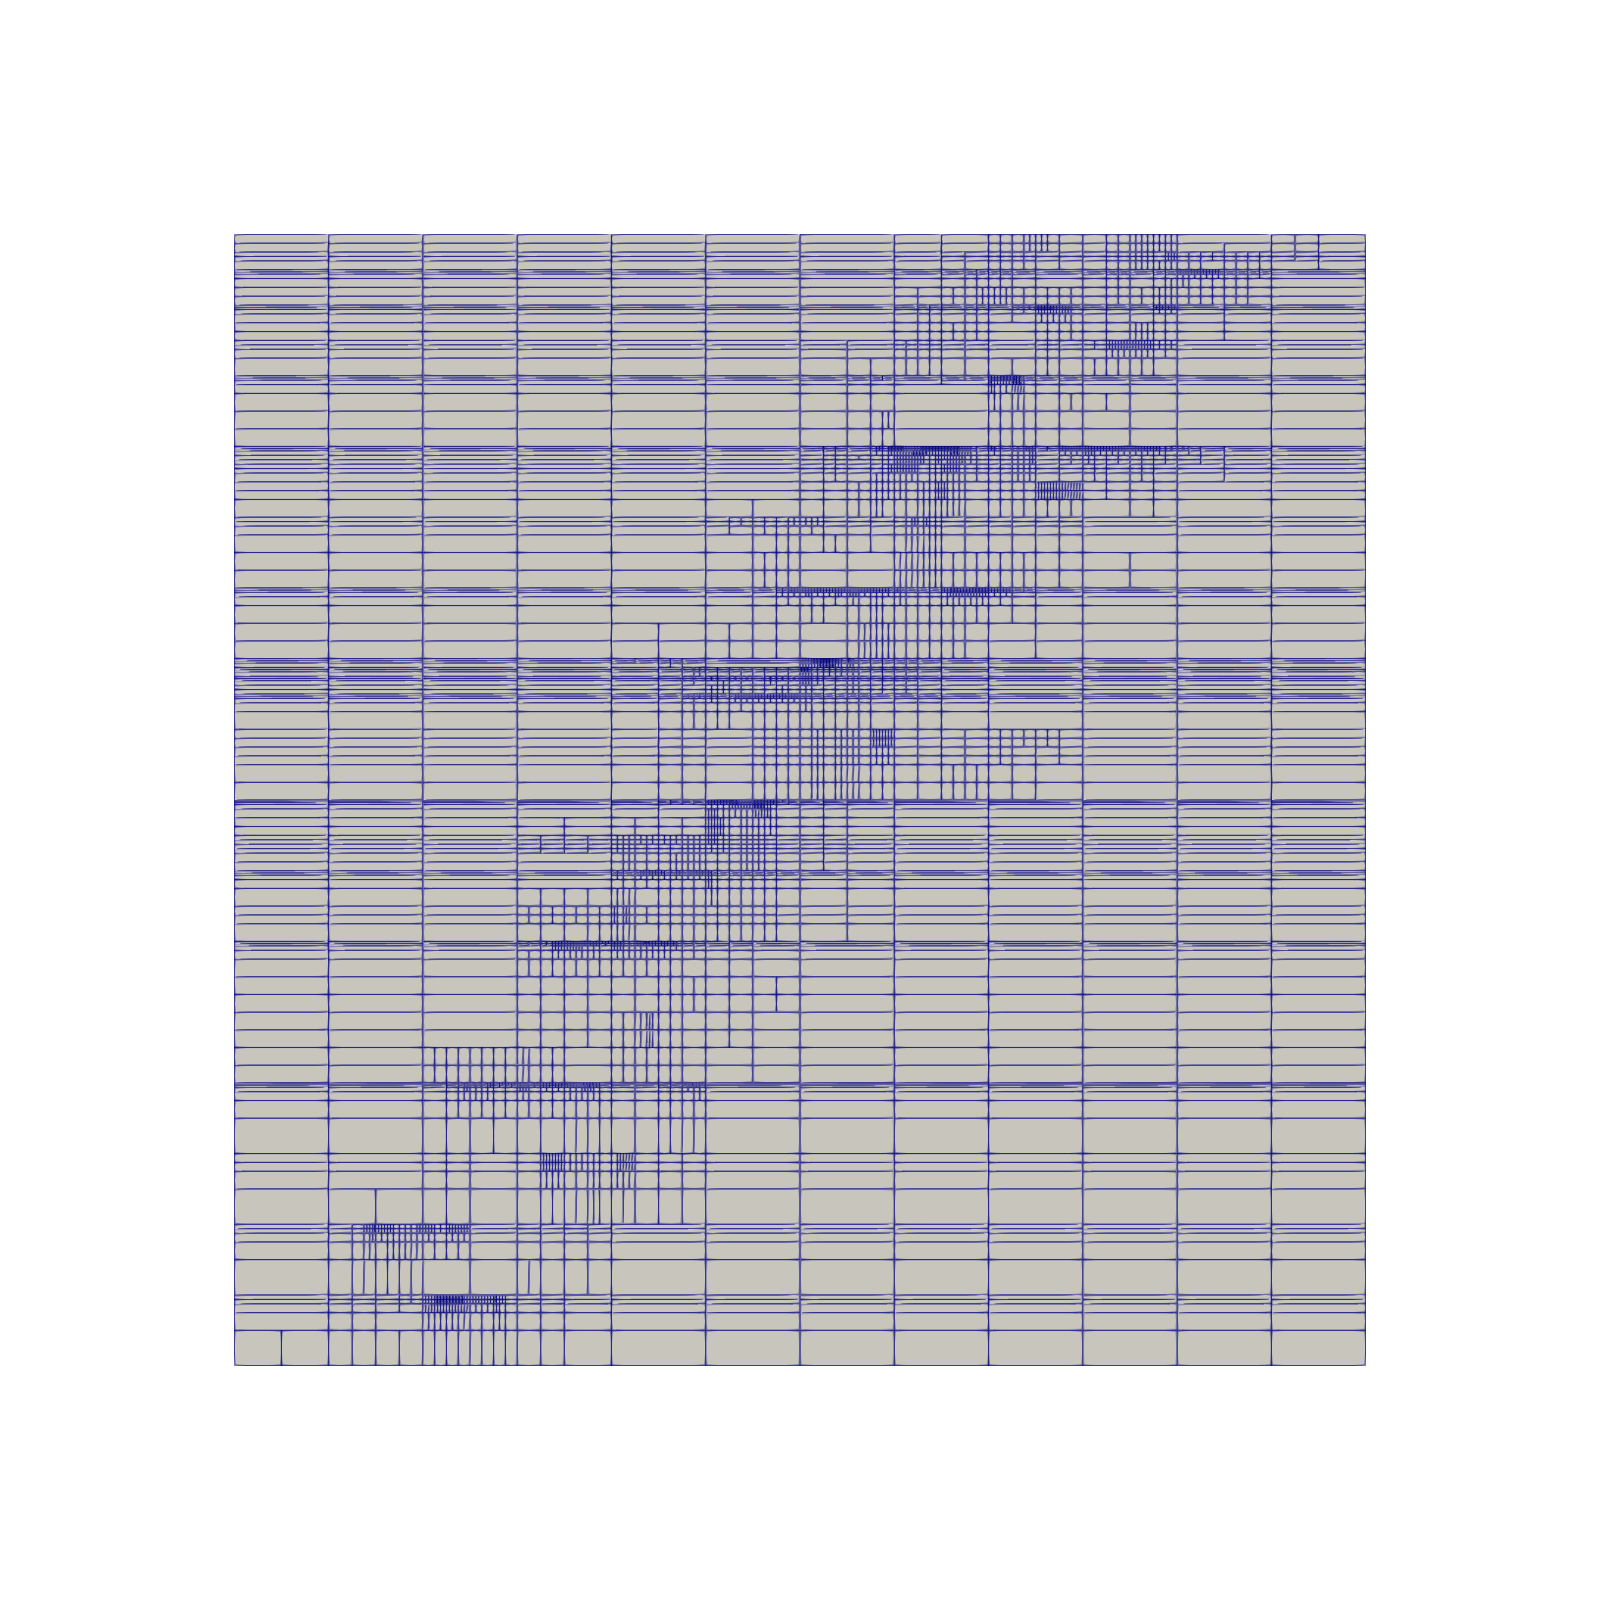
\includegraphics[
      width=\linewidth
    ]{figures/advection_diffusion_1d/mesh_x080_iter.0008.png}
    \caption{Iteration 8.}
  \end{subfigure}
  \caption{Evolution of the space--time mesh for the Gaussian detector centred at $x_d=0.8$.}
  \label{fig:advection-diffusion-evolution}
\end{figure}

\cref{fig:advection-diffusion-initial-marks} compares the space--time cells selected during the first adaptive iteration. For the detector at $x_d=0.7$, the marked cells form a relatively continuous diagonal band towards the trailing side of the pulse. Fifteen space--time cells are selected, distributed over eight time slabs. For the central detector at $x_d=0.8$, the marked set is more concentrated: the bulk marking criterion is satisfied using only ten cells, and only two time slabs satisfy the temporal refinement criterion. In contrast, the detector at $x_d=0.9$ produces a broader marked region at later times, shifted towards the leading side of the pulse. Sixteen cells are selected and four time slabs are marked for temporal refinement.
\begin{figure}[h]
  \centering
  % space--time axis
  \begin{subfigure}[h]{0.05\textwidth}
    \centering
    \begin{tikzpicture}[>=latex, line width=0.6pt, scale=0.8]
      \draw[->] (0,0) -- (0,0.6) node[above=1pt] {$t$};
      \draw[->] (0,0) -- (0.6,0) node[below=1pt] {$x$};
    \end{tikzpicture}
    \vspace{-2em}
    \captionsetup{labelformat=empty}
    \caption{}
  \end{subfigure}
  \hfill
  \begin{subfigure}[h]{0.30\textwidth}
    \centering
    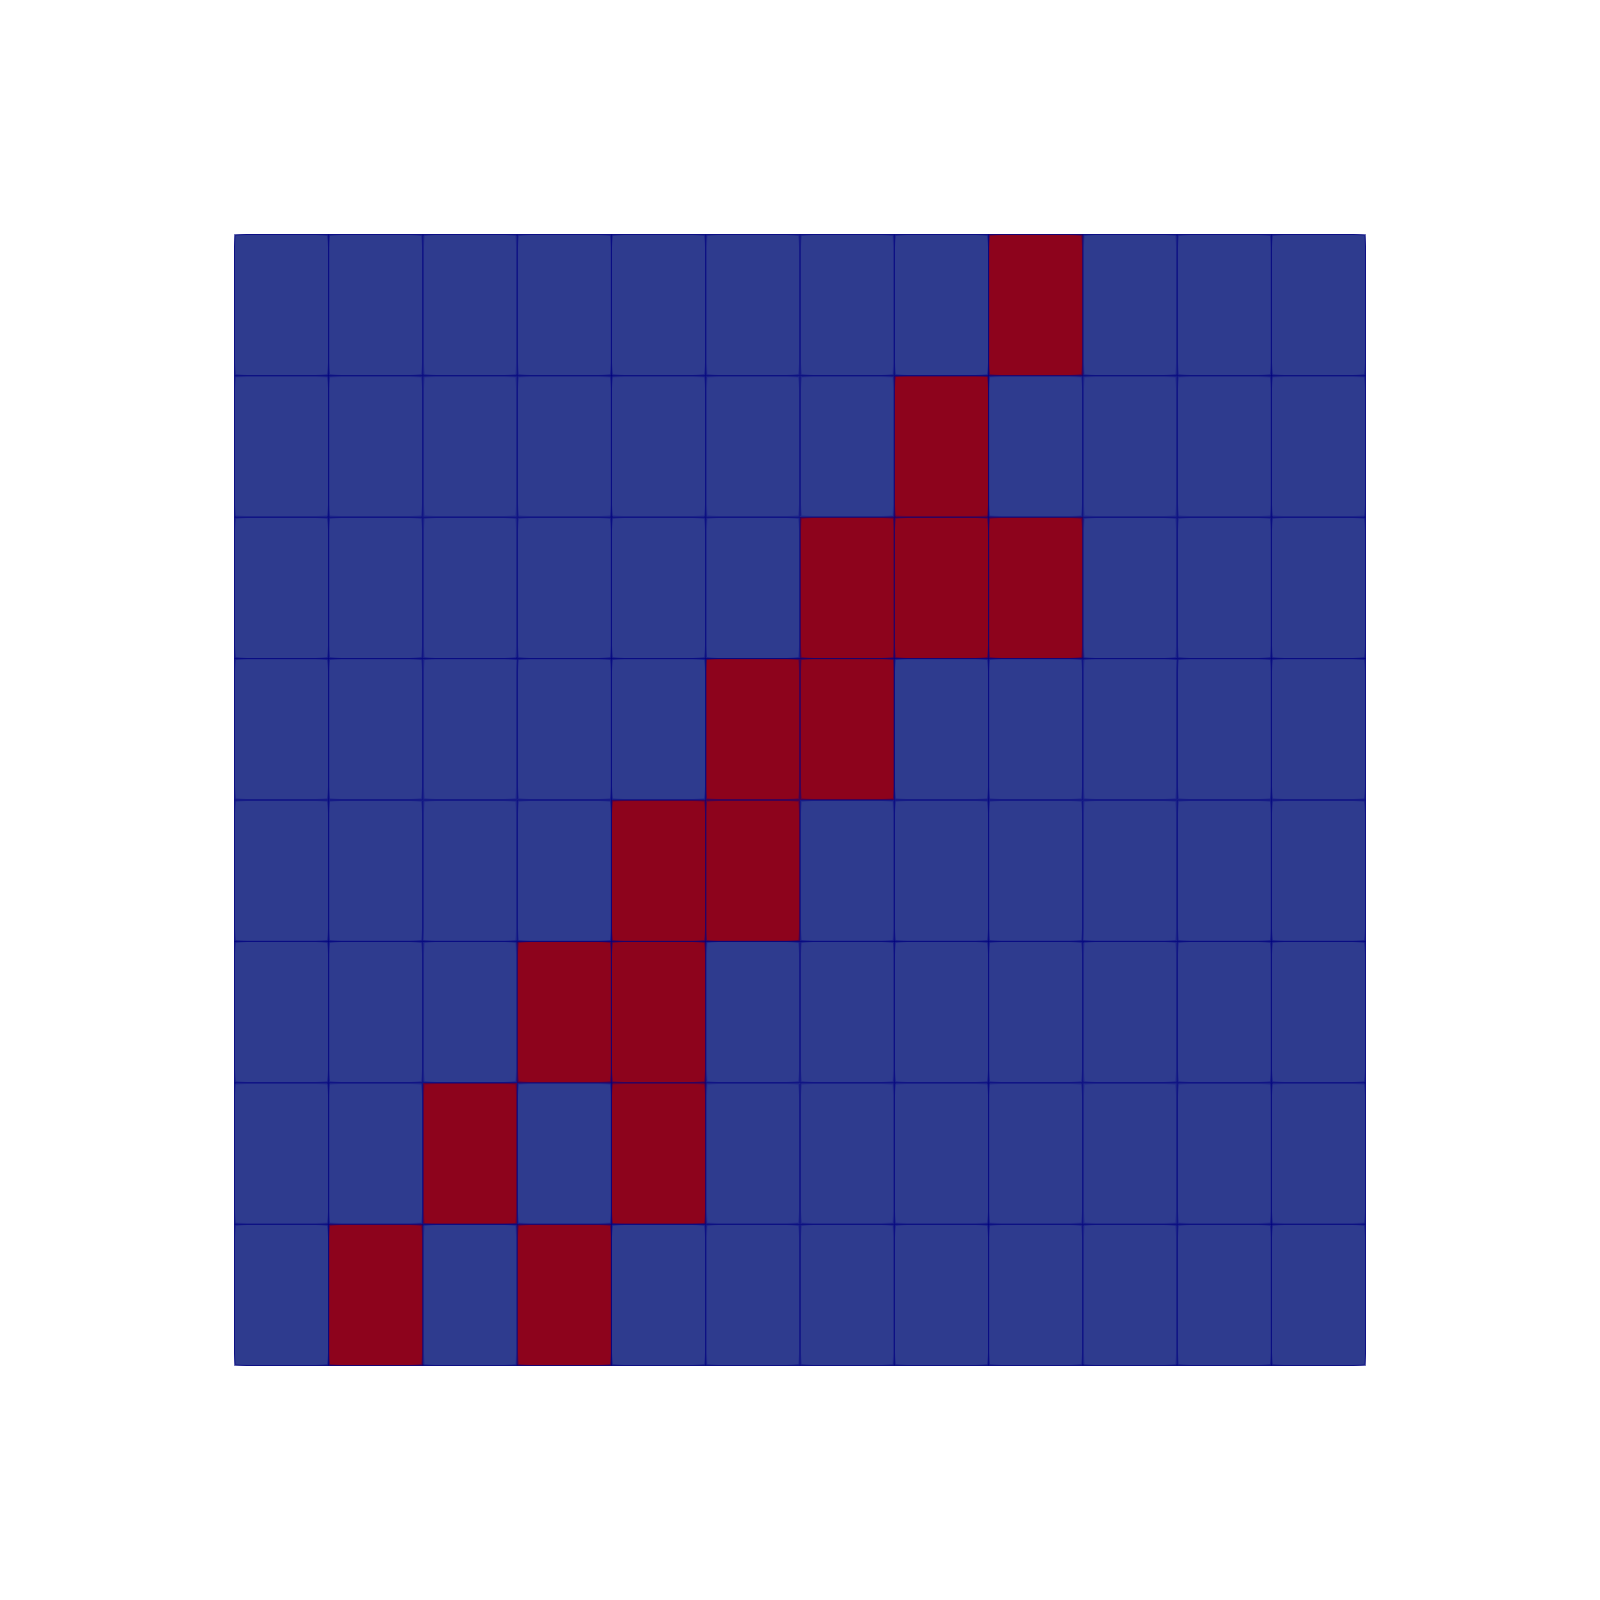
\includegraphics[
      width=\linewidth
    ]{figures/advection_diffusion_1d/marked_x070_iter0.png}
    \caption{$x_d=0.7$.}
  \end{subfigure}
  \hfill
  \begin{subfigure}[h]{0.30\textwidth}
    \centering
    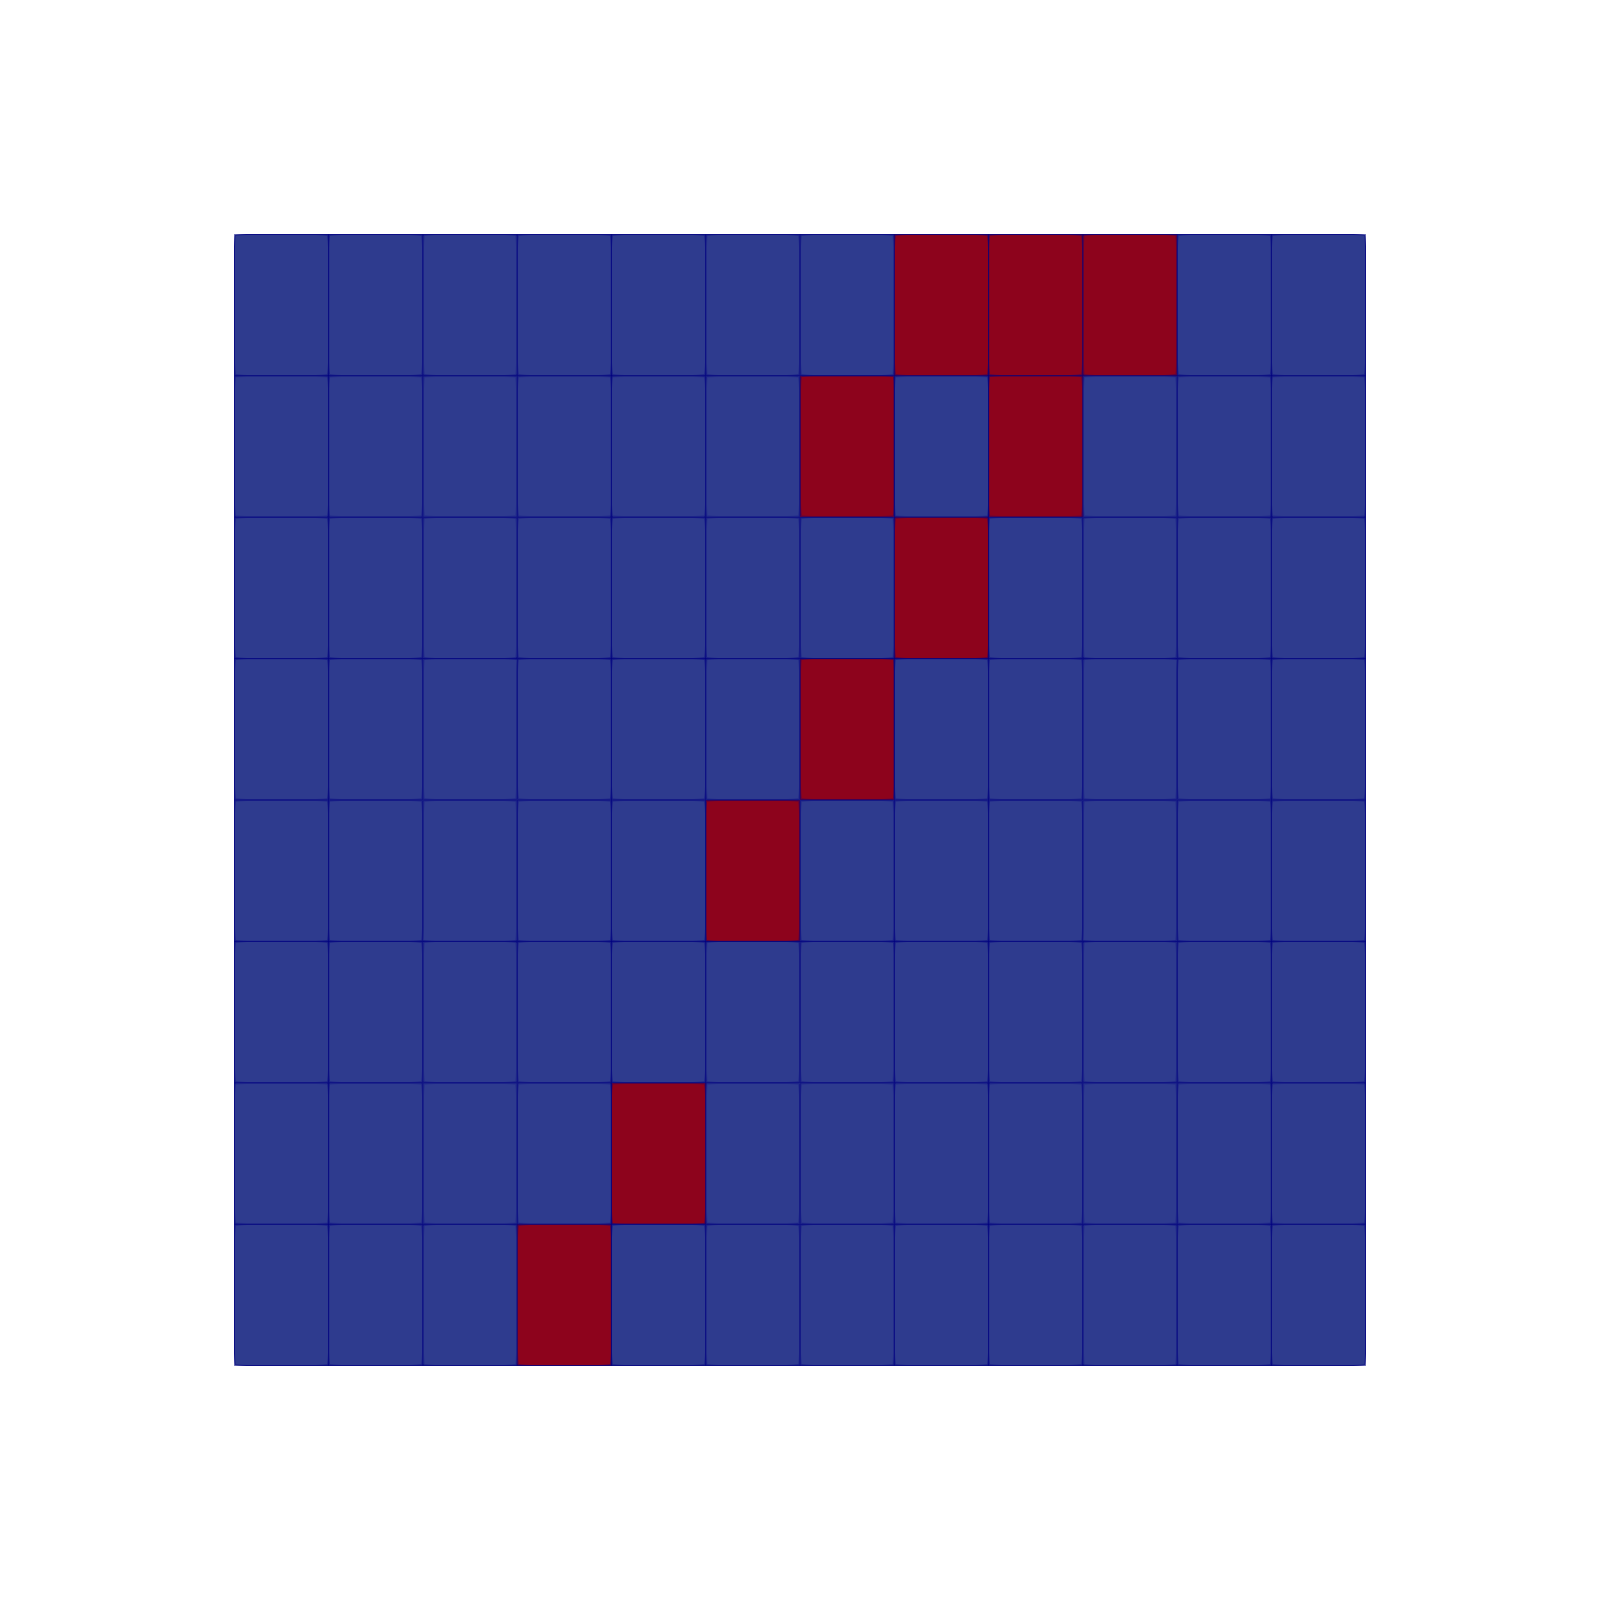
\includegraphics[
      width=\linewidth
    ]{figures/advection_diffusion_1d/marked_x080_iter0.png}
    \caption{$x_d=0.8$.}
  \end{subfigure}
  \hfill
  \begin{subfigure}[h]{0.30\textwidth}
    \centering
    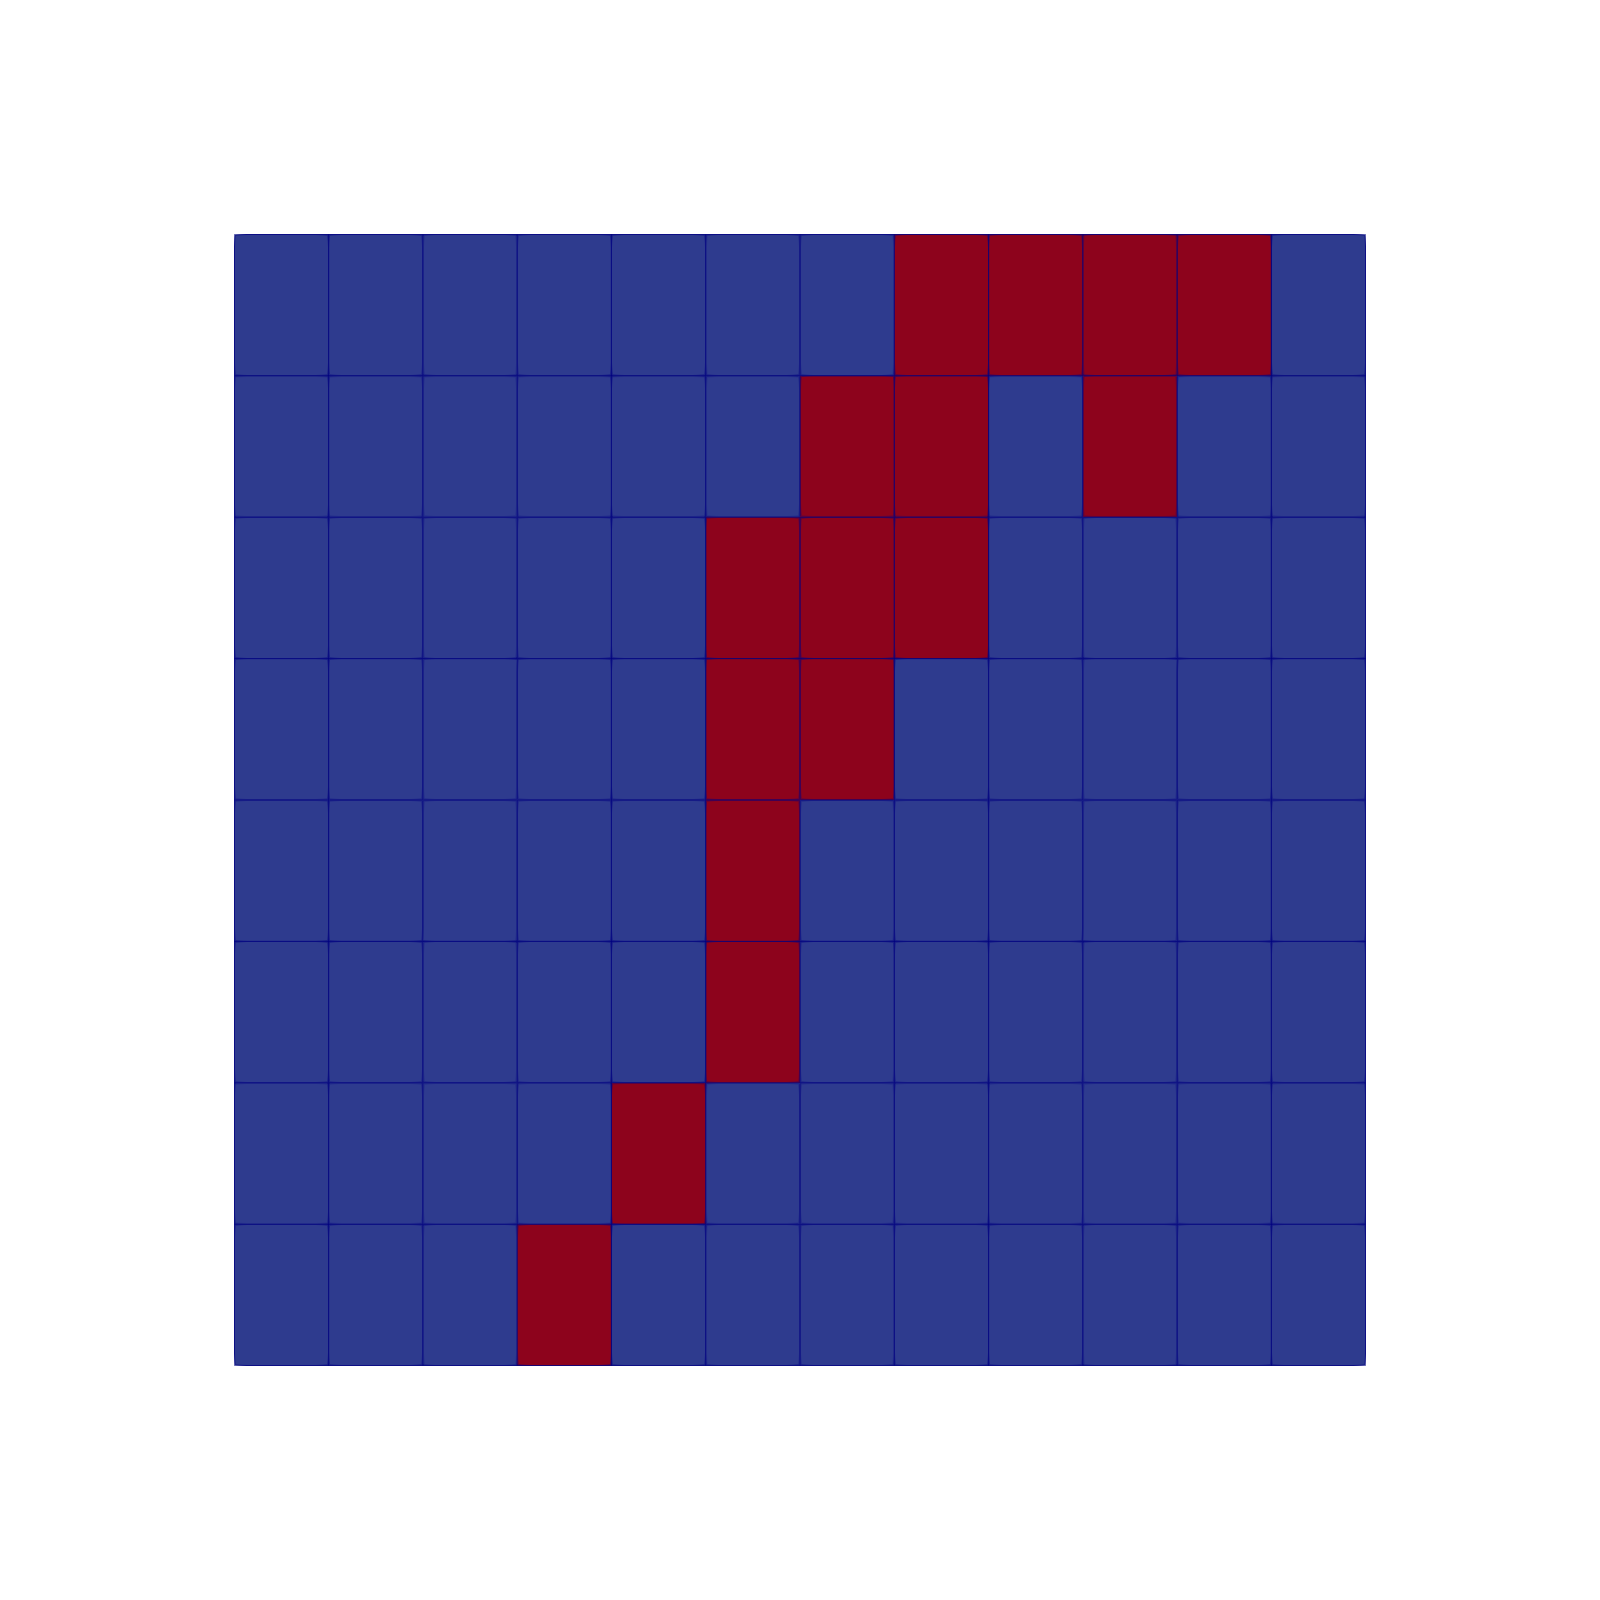
\includegraphics[
      width=\linewidth
    ]{figures/advection_diffusion_1d/marked_x090_iter0.png}
    \caption{$x_d=0.9$.}
  \end{subfigure}
  \caption{Space--time cells marked during the first adaptive iteration for Gaussian terminal sensors centred at three different locations $x_d$.}
  \label{fig:advection-diffusion-initial-marks}
\end{figure}

The final adapted meshes are compared in~\cref{fig:advection-diffusion-final-meshes}. Changing the detector location modifies the shape and terminal destination of the refined space--time tube. For $x_d=0.7$, refinement follows a comparatively continuous diagonal path towards the trailing part of the pulse. For $x_d=0.8$, the refined region remains concentrated around the central pulse trajectory as shown in ~\cref{fig:advection-diffusion-exact}. For $x_d=0.9$, the late-time refinement is shifted further to the right and bends towards the leading part of the pulse. When traced backwards in time, the three refined regions return towards the common initial pulse location near $x_0=0.2$. This demonstrates that the terminal sensor affects through the backward propagation of the dual weight, as expected.

\begin{figure}[h]
  \centering
  % space--time axis
  \begin{subfigure}[h]{0.05\textwidth}
    \centering
    \begin{tikzpicture}[>=latex, line width=0.6pt, scale=0.8]
      \draw[->] (0,0) -- (0,0.6) node[above=1pt] {$t$};
      \draw[->] (0,0) -- (0.6,0) node[below=1pt] {$x$};
    \end{tikzpicture}
    \vspace{-2em}
    \captionsetup{labelformat=empty}
    \caption{}
  \end{subfigure}
  \hfill
  \begin{subfigure}[h]{0.30\textwidth}
    \centering
    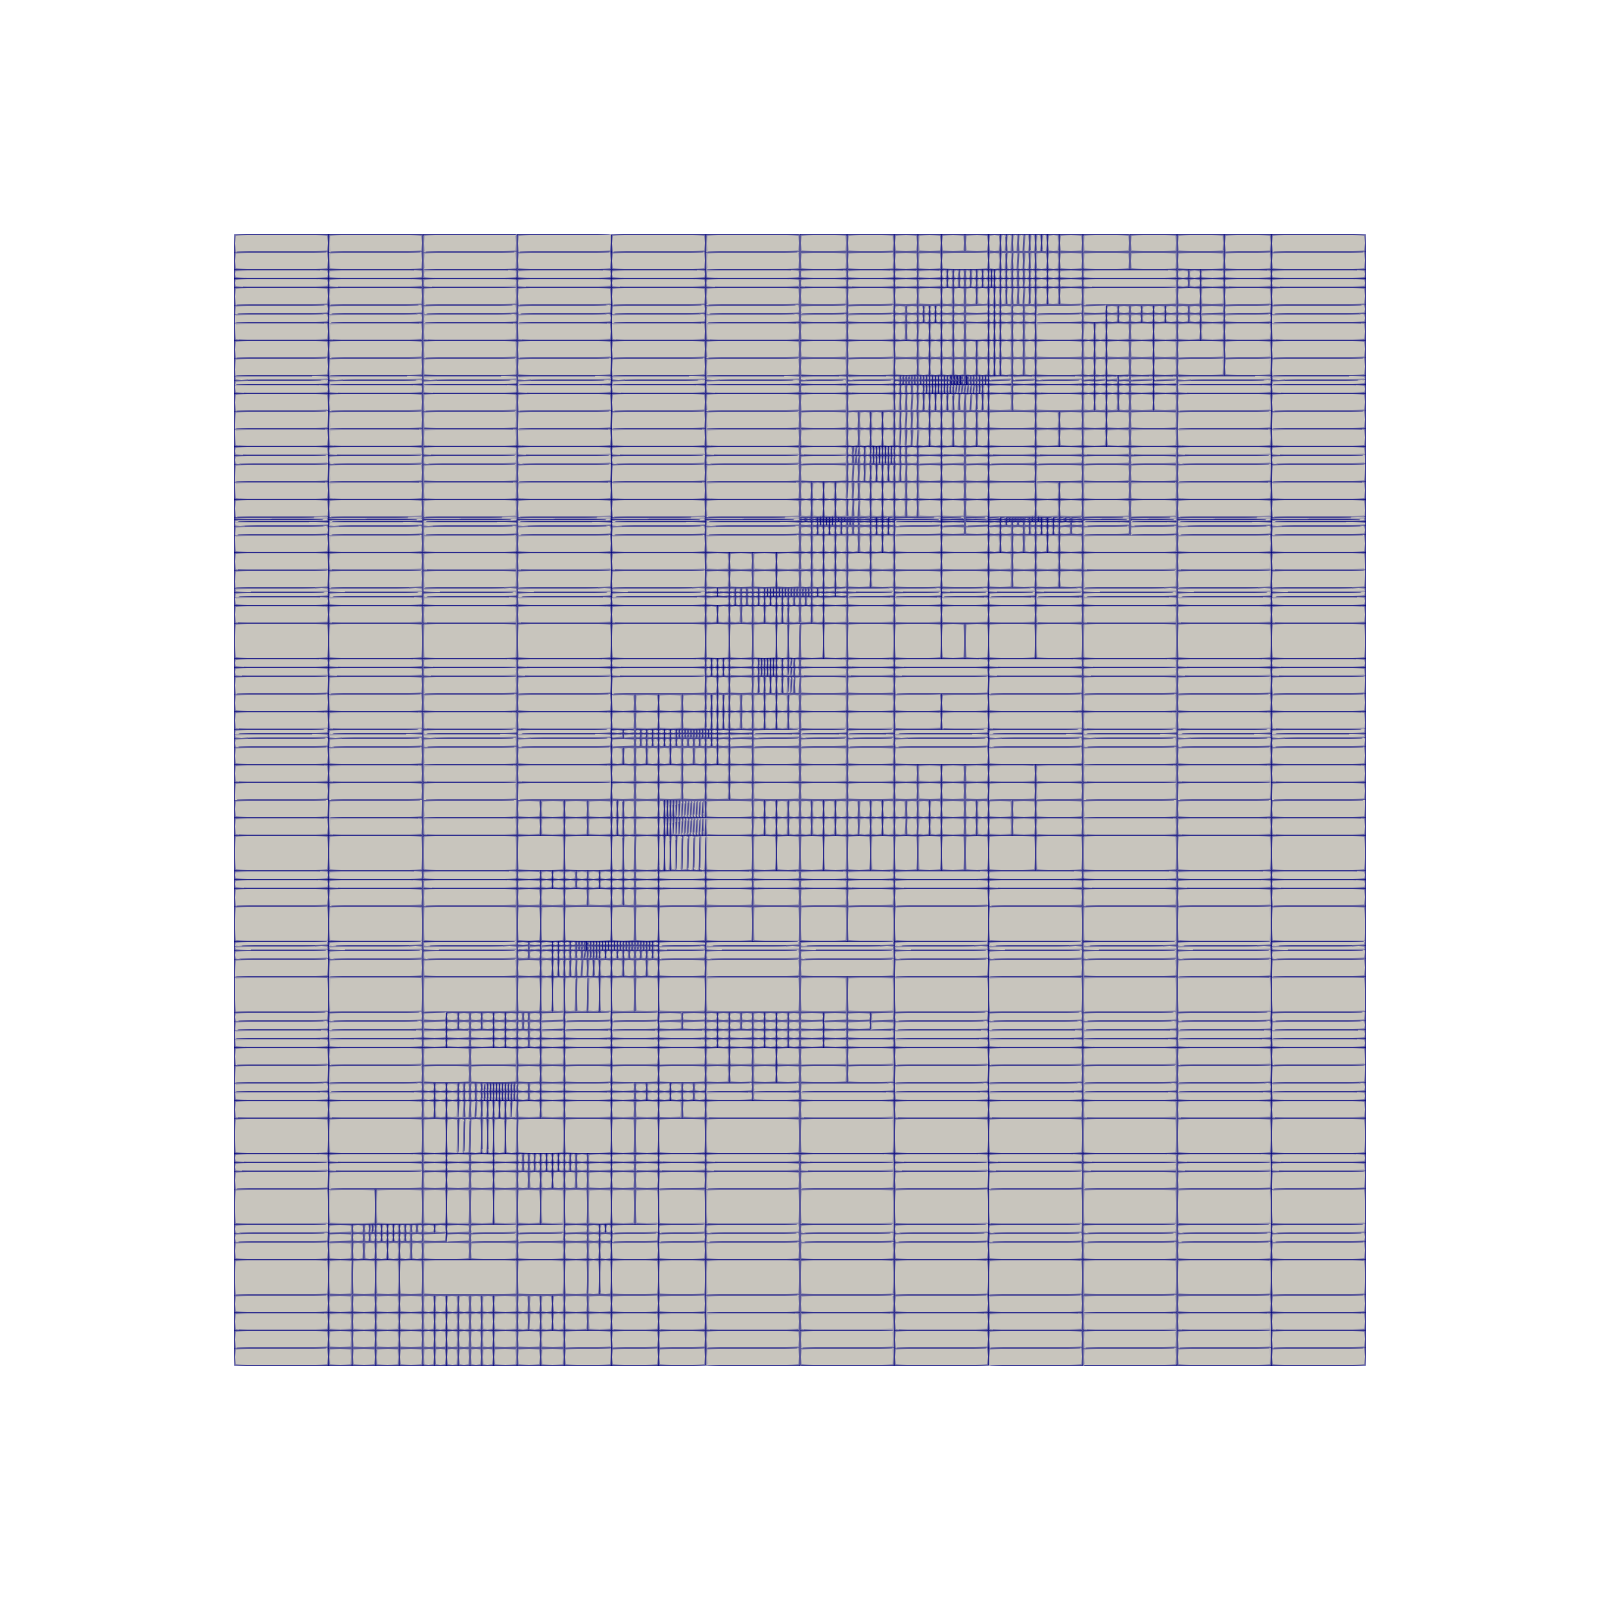
\includegraphics[
      width=\linewidth
    ]{figures/advection_diffusion_1d/mesh_x070_iter6.png}
    \caption{$x_d=0.7$.}
  \end{subfigure}
  \hfill
  \begin{subfigure}[h]{0.30\textwidth}
    \centering
    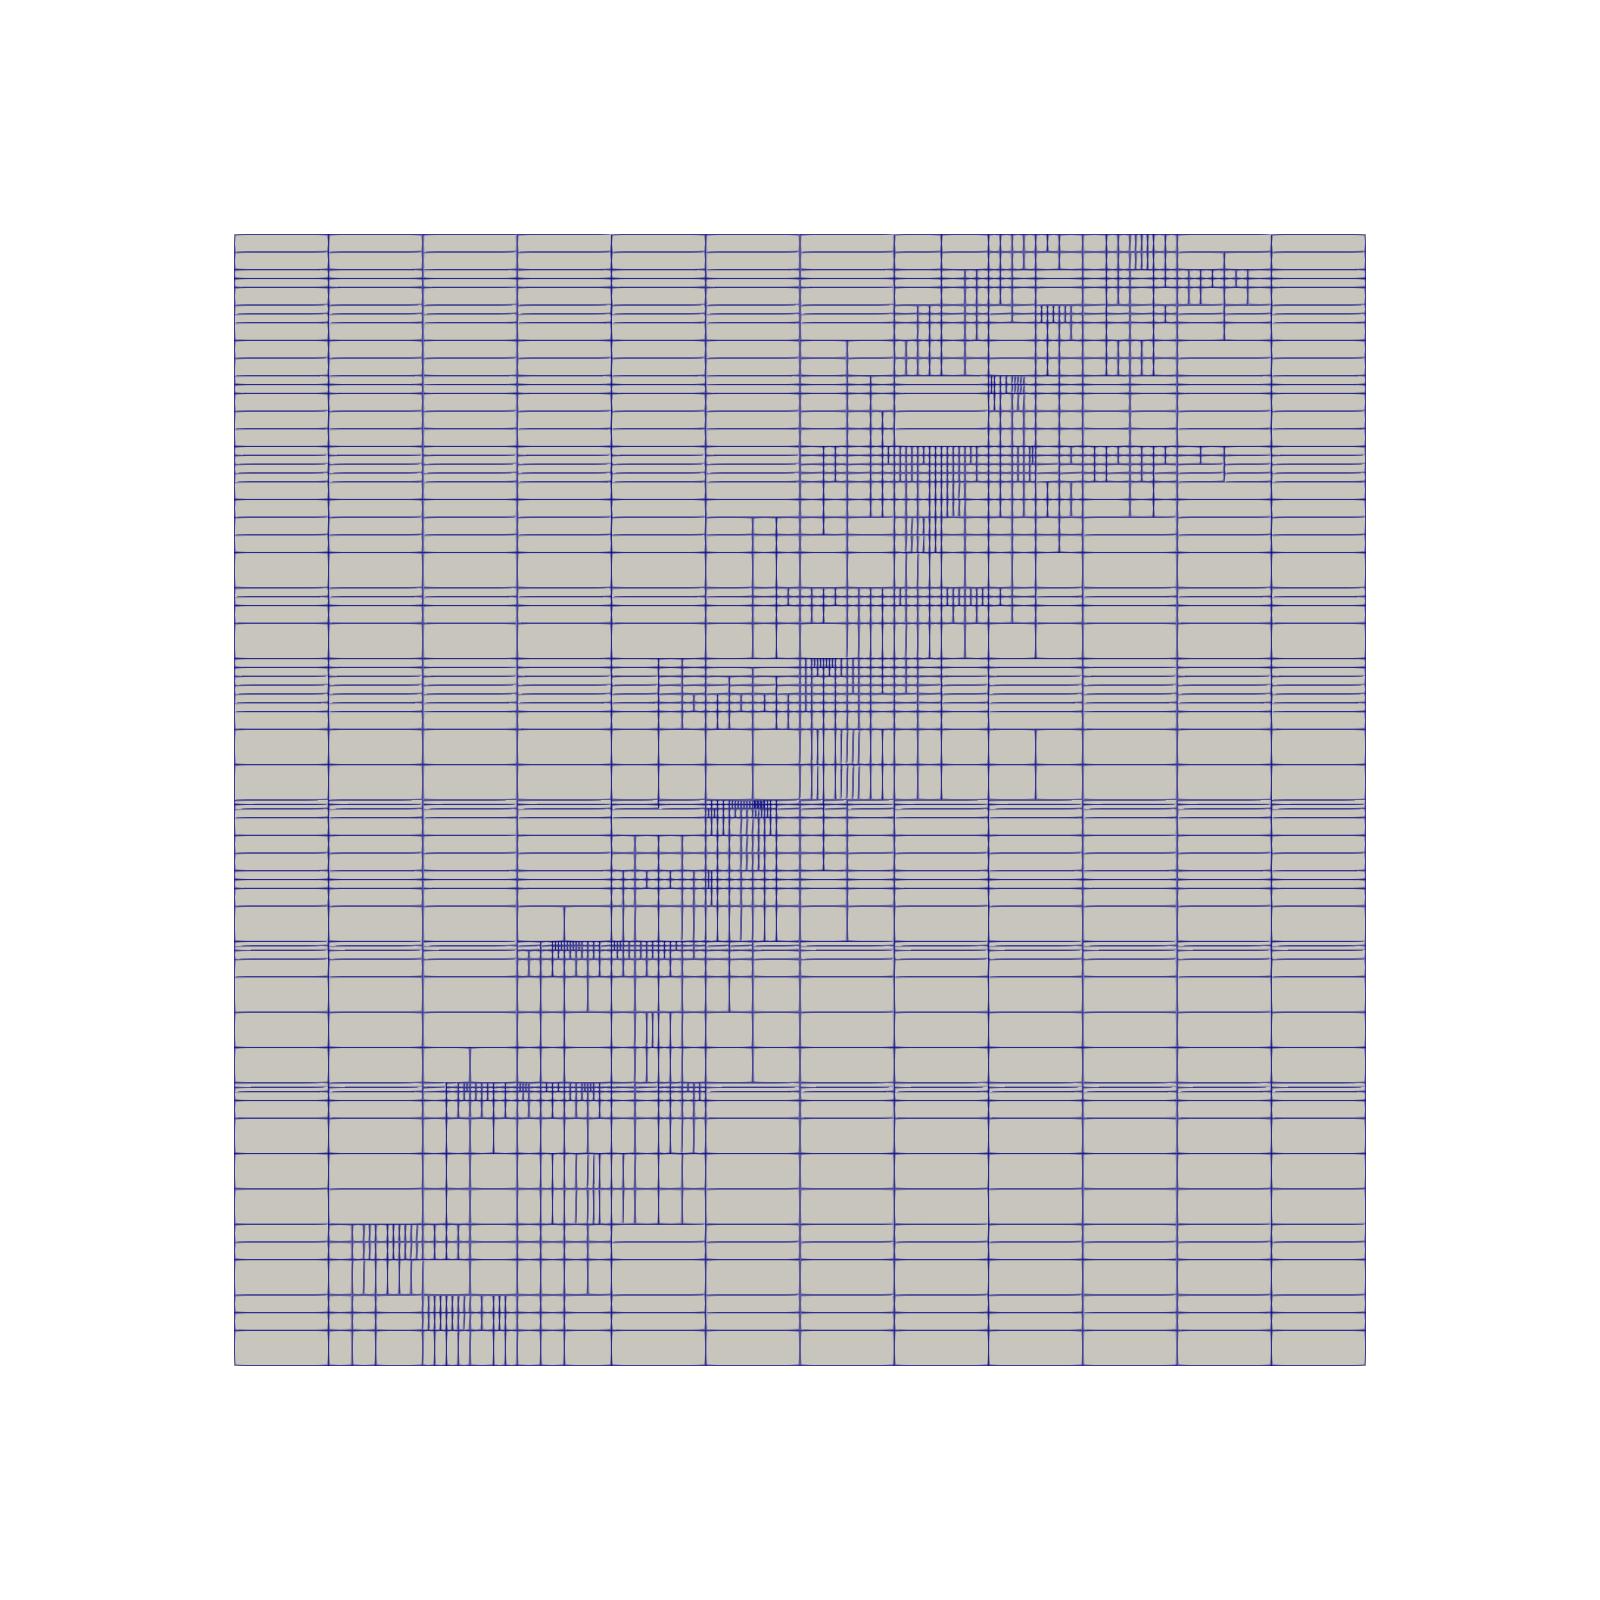
\includegraphics[
      width=\linewidth
    ]{figures/advection_diffusion_1d/mesh_x080_iter6.png}
    \caption{$x_d=0.8$.}
  \end{subfigure}
  \hfill
  \begin{subfigure}[h]{0.30\textwidth}
    \centering
    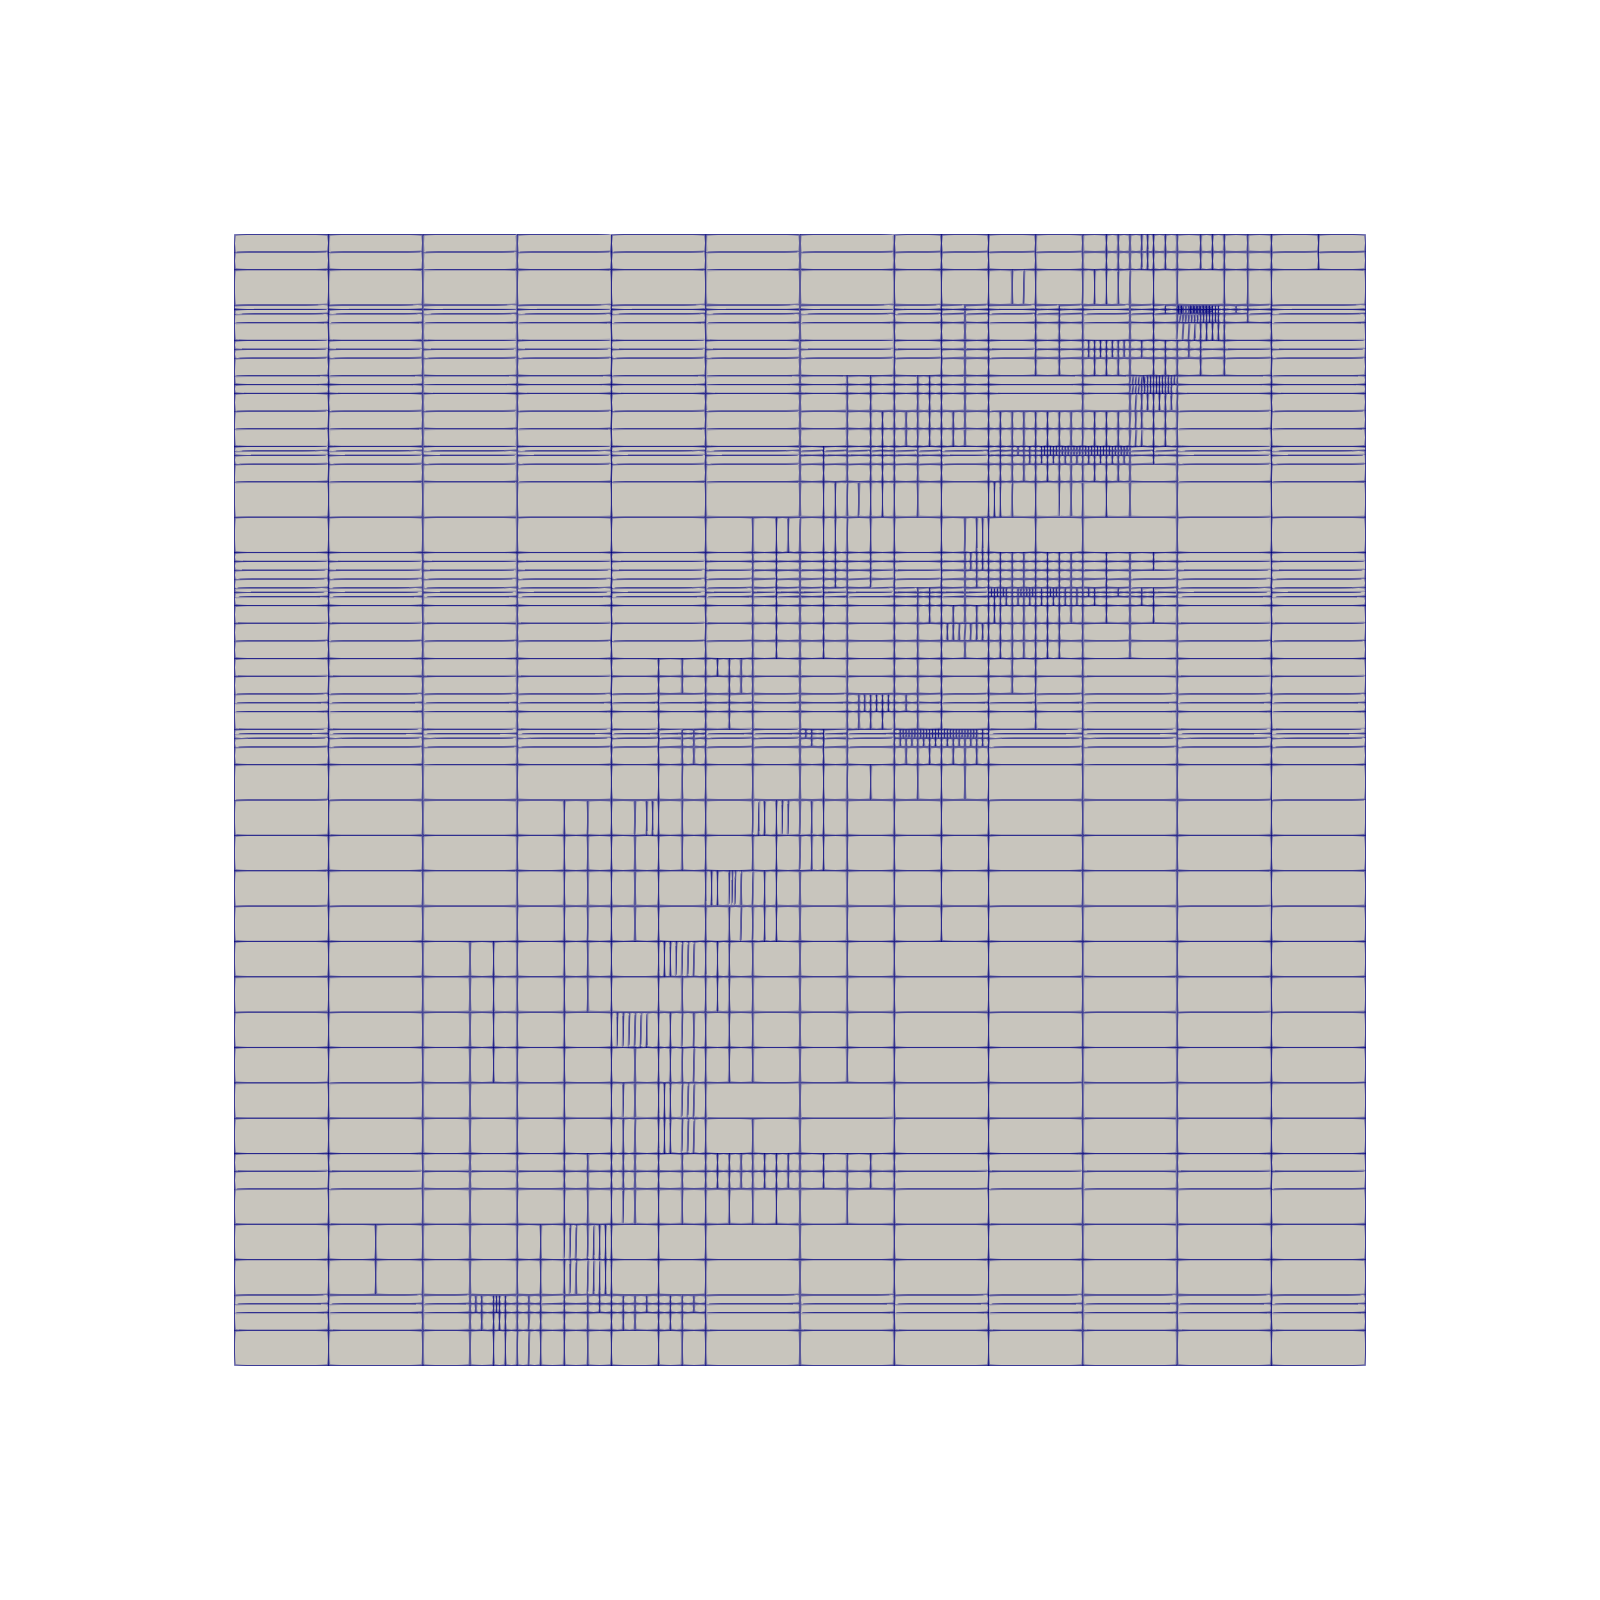
\includegraphics[
      width=\linewidth
    ]{figures/advection_diffusion_1d/mesh_x090_iter6.png}
    \caption{$x_d=0.9$.}
  \end{subfigure}
  \caption{Final adapted space--time meshes for Gaussian terminal sensors centred at $x_d=0.7$, $0.8$, and $0.9$.}
  \label{fig:advection-diffusion-final-meshes}
\end{figure}

% \begin{table}[htbp]
%   \centering
%   \caption{
%     Global DWR estimator and signed effectivity index for the three
%     Gaussian detector locations.
%   }
%   \label{tab:advection-diffusion-effectivity}
%   \small
%   \begin{tabular}{
%     c
%     rr
%     rr
%     rr
%   }
%     \toprule
%     & \multicolumn{2}{c}{$x_d=0.7$}
%     & \multicolumn{2}{c}{$x_d=0.8$}
%     & \multicolumn{2}{c}{$x_d=0.9$} \\
%     \cmidrule(lr){2-3}
%     \cmidrule(lr){4-5}
%     \cmidrule(lr){6-7}
%     Iteration
%     & $\eta$ & $I_{\mathrm{eff}}$
%     & $\eta$ & $I_{\mathrm{eff}}$
%     & $\eta$ & $I_{\mathrm{eff}}$ \\
%     \midrule
%     0
%     & $ 6.876{\times}10^{-4}$ & $ 1.681$
%     & $ 6.573{\times}10^{-3}$ & $ 0.962$
%     & $ 1.992{\times}10^{-3}$ & $ 0.887$ \\
%     1
%     & $-8.010{\times}10^{-5}$ & $ 0.116$
%     & $ 4.808{\times}10^{-3}$ & $ 0.780$
%     & $ 1.799{\times}10^{-3}$ & $ 0.814$ \\
%     2
%     & $ 9.895{\times}10^{-6}$ & $-0.016$
%     & $ 3.559{\times}10^{-3}$ & $ 0.737$
%     & $ 1.633{\times}10^{-3}$ & $ 1.113$ \\
%     3
%     & $-1.757{\times}10^{-4}$ & $ 0.315$
%     & $ 2.763{\times}10^{-3}$ & $ 0.697$
%     & $ 1.179{\times}10^{-3}$ & $ 0.955$ \\
%     4
%     & $-5.041{\times}10^{-5}$ & $ 0.081$
%     & $ 2.326{\times}10^{-3}$ & $ 0.875$
%     & $ 7.867{\times}10^{-4}$ & $ 0.812$ \\
%     5
%     & $ 1.795{\times}10^{-7}$ & $-0.000$
%     & $ 1.975{\times}10^{-3}$ & $ 1.006$
%     & $ 7.576{\times}10^{-4}$ & $ 0.887$ \\
%     6
%     & $-6.338{\times}10^{-5}$ & $ 0.139$
%     & $ 1.607{\times}10^{-3}$ & $ 1.309$
%     & $ 6.769{\times}10^{-4}$ & $ 0.752$ \\
%     \bottomrule
%   \end{tabular}
% \end{table}
